\documentclass{cumcmthesis}
%\documentclass[withoutpreface,bwprint]{cumcmthesis} %去掉封面与编号页
\title{TITLE}
\tihao{A}            % 题号
\baominghao{4321}    % 报名号
\schoolname{你的大学}
\membera{成员A}
\memberb{成员B}
\memberc{成员C}
\supervisor{指导老师}
\yearinput{2017}     % 年
\monthinput{08}      % 月
\dayinput{22}        % 日
\usepackage{float}
\usepackage{listings}
\usepackage{tikz}

\begin{document}
	\maketitle
	\begin{abstract}


		\keywords{关键词1\quad  关键词2\quad   关键词3}
	\end{abstract}

	\section{问题重述}


	\section{问题分析}

	
	\section{符号说明}
	\begin{center}
		\begin{tabular}{ccc}
			\hline
			\makebox[0.3\textwidth][c]{符号}	& 
			\makebox[0.4\textwidth][c]{说明}	&
			\makebox[0.3\textwidth][c]{单位} \\ \hline
			$S$	    & 被观测的天体            &    \\ 
			$\beta$	& 角度1                  & $^\circ$  \\ \hline
		\end{tabular}
	\end{center}
	

	\section{模型假设}
	
	
	\section{模型建立与求解}
	
	
	\section{模型评价}
	
	
	\newpage            % 换页
	\section{其他模板}
	\subsection{}       % 子标题
	\subsubsection{}


	
	\[					% 占行公式
	\alpha=28^\circ		% 角度表示
	\]
	
	
	
	\begin{equation}	% 带编号的公式
		E=mc^2
		\label{energy}
	\end{equation}  \par 

	
	
	use equation \cref{energy}.   \par    % 引用上述公式
	
	
	
	according to reference \cite{bib:one}.    \par    % 引用参考文献
	
	
	
	this is a footnote.\footnote{text}  \par      % 脚注
	
	
	
	text spells tike this -- \texttt{result.xlsx}.   % 文件表示
	
	
	
	\begin{table}[H]   % 三线表
		\begin{center}
			\begin{tabular}{cc}
				\hline
				\makebox[0.4\textwidth][c]{$key$} &
				\makebox[0.4\textwidth][c]{$value$} \\ \hline
				$a$   &   $b$ \\
				$c$   &   $d$ \\  \hline
			\end{tabular}
		\end{center}
		\caption{三线表模板}
	\end{table}
	
	
	
	\begin{figure}[H]   % 图
		\centering
		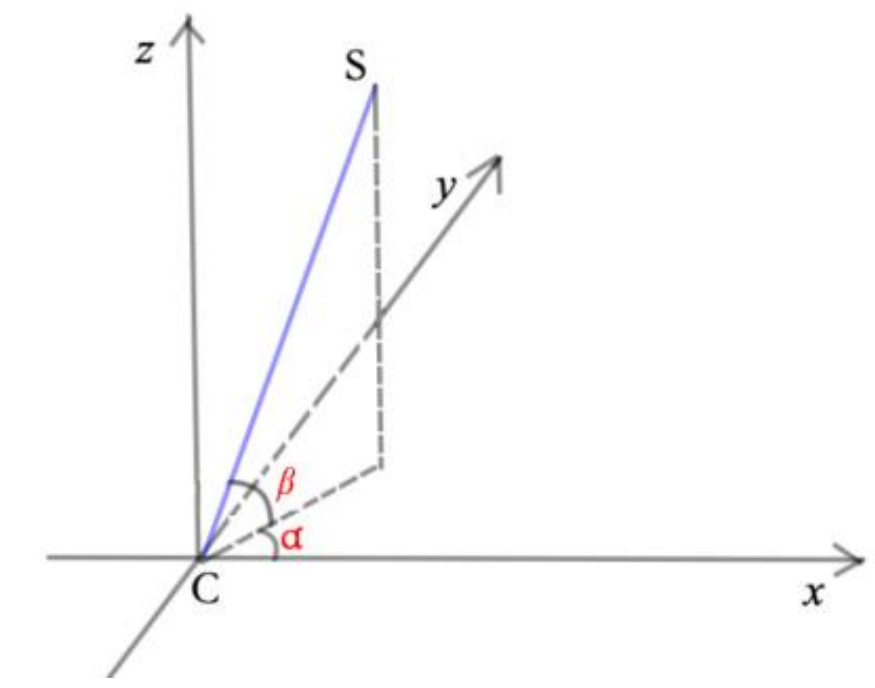
\includegraphics[width=0.6\textwidth]{system}
		\caption{图模板}
		\label{system}
	\end{figure}
	
	
	
	\begin{figure}[H]   % 多图并排
		\centering
		\begin{minipage}[c]{0.4\textwidth}
			\centering
			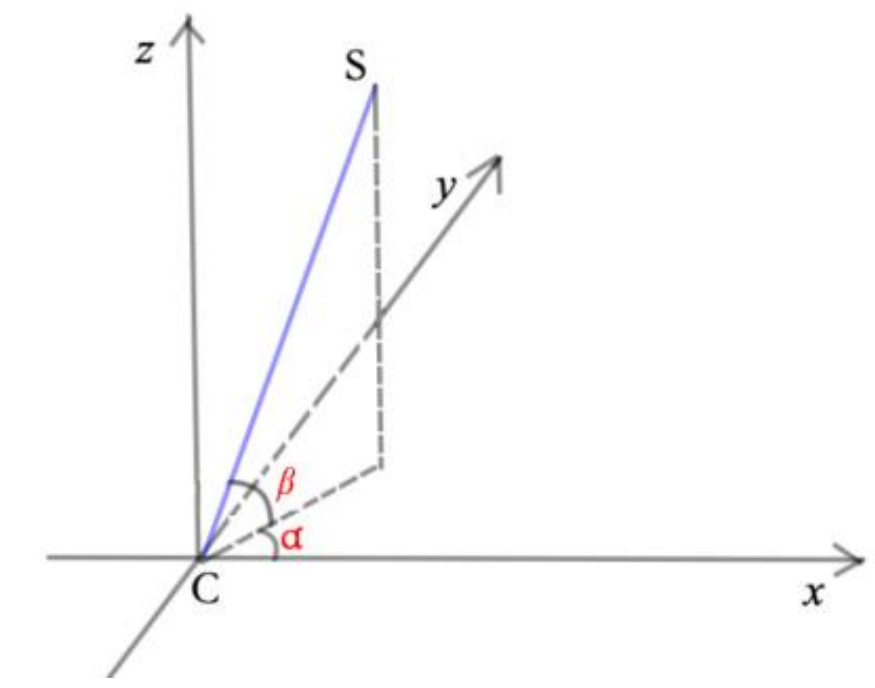
\includegraphics[width=0.95\textwidth]{system}
			\subcaption{并排图1}
			\label{fig:sample-figure-a}
		\end{minipage}
		\begin{minipage}[c]{0.4\textwidth}
			\centering
			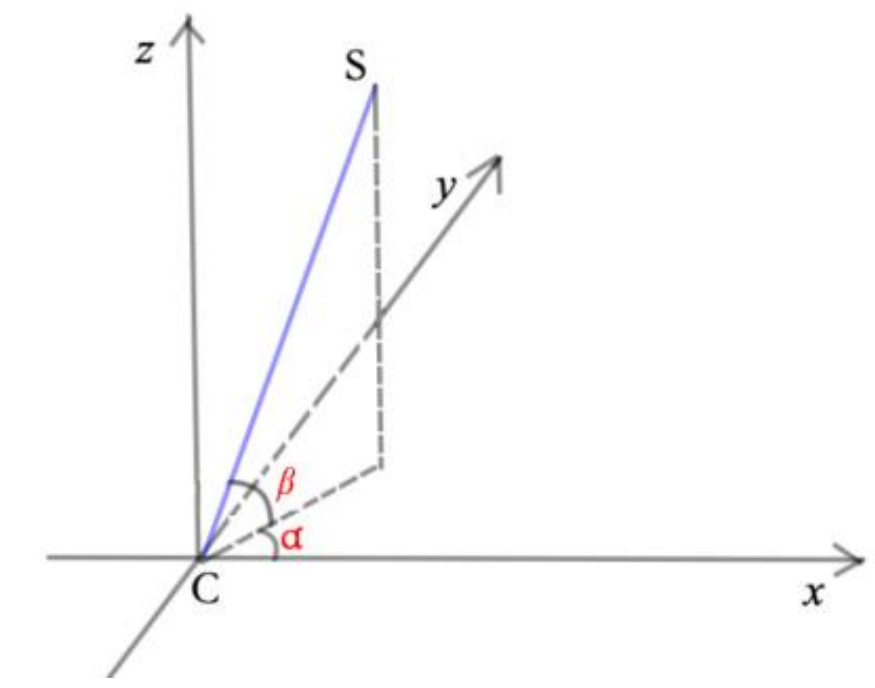
\includegraphics[width=0.95\textwidth]{system}
			\subcaption{并排图2}
			\label{fig:sample-figure-b}
		\end{minipage}
		\caption{多图并排示例}
		\label{fig:sample-figure}
	\end{figure}
	
	
	
	\noindent noindent example   \par % 顶格 取消换行 
		
		
	
	\begin{itemize}   % 顶格序号子项 1.  2.
		\item[1.]11111
		\item[2.]22222
	\end{itemize}   \par
	
	
	
	$\overrightarrow{AB}$     % 向量表示
	
	
	
	\underline{underline}    % 下划线
	
	
	
	\[
	{\rm{arcsin}} x          % 取消斜体表示
	\]
	
	
	
	\[
	S _{0}^{\prime}          % 上下标
	\]
	
	
	
	\[
	\int _{0} ^{1} f(x) {\rm{d}} x    % 含上下限的积分表示
	\]
	
	
	
	\[
	\sum _0 ^3 |x^2|       %  含上下限的求和符号表示
	\]
	
	

	\[
		f(x)=					% 大括号的表示一(含左等号)
		\begin{cases}
			\rho = \pi   \\
			\theta = \alpha
		\end{cases}
	\]
	
	
	
	\[
		\begin{cases}           % 大括号的表示二(不含左等号)
			\rho = \frac{2(F-l)}{1-{\rm{cos}}\theta} \\    % 分数表示    字符返回正体
			L=\sqrt{\rho^2 - 2 \cdot CP \times AB}         % 点乘       叉乘
		\end{cases}
	\]
	
	
	\[
		A\circ B				%  圆乘
	\]

	
	
	
	\[
		\mathbf {X} = \left(            % 矩阵表示
		\begin{array}{cccc}
		
			x_{11} & x_{12} & \vdots & x_{14}\\
			x_{11} & x_{12} & \vdots & x_{14}\\
			\cdots & \ldots & \ddots & \ldots\\
			x_{11} & x_{12} & \vdots & x_{14}\\
		
		\end{array} \right)
	\]

	
	\newpage
	\begin{thebibliography}{9} % 参考文献
		\bibitem{bib:one}
		writer.
		\newblock bookname\allowbreak [J].
		\newblock xx出版社,Beijing,2017.
	\end{thebibliography}
	\begin{appendices}  
		\begin{lstlisting}[language={python}]  
			print("hello world")
		\end{lstlisting}  % 此处粘贴python代码
	\end{appendices}
\end{document}